\documentclass[a4paper,12pt]{article} %style de document
\usepackage[utf8]{inputenc}
\usepackage{hyperref}
\usepackage{url}
\usepackage[T1]{fontenc}
\usepackage[a4paper]{geometry}
\usepackage{lipsum}
%\usepackage[french]{babel}
\usepackage[T1]{fontenc} %encodage de la police
\usepackage{graphicx}



\usepackage{listings}
\usepackage{xcolor}
\usepackage{xparse}



\usepackage{caption} 
\captionsetup[figure]{font={small, sf},labelformat=empty}

\title{\vspace{\fill}CoreWar\vspace{\fill}}


\author{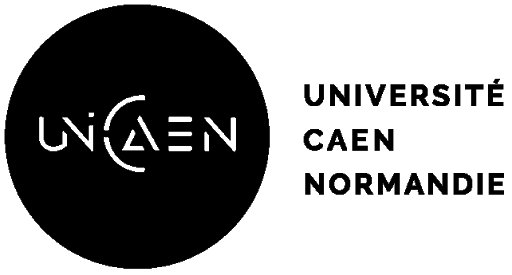
\includegraphics[scale=0.3]{images/unicaen.png} \\
		Alexander Camatchy\\Alix Danvy\\Mateo Delerue\\Abdoulaye Fofana\\\\
        L2 informatique\\
        Groupe 3A \\
        UNICAEN}
\date{Avril 2022}

\NewDocumentCommand{\code}{v}{
	\texttt{\textcolor{orange}{#1}}
}

\begin{document}

\maketitle

\newpage

\tableofcontents

\newpage
\section{Introduction}
\subsection{CoreWar}
CoreWar est un jeu de programmation où plusieurs programmes s'affrontent au sein d'une mémoire virtuelle. Les programmes sont écrits en RedCode, un langage proche de l'assembler. Le CoreWar que nous avons implémenté suit la norme ICWS-88. Ce standard définit 11 instructions et 5 modes d'adressage (octothorpe, direct, indirect, pré-incrémente et pré-décrémente). Les programmes peuvent écrire dans des cases mémoires, effectuer des opérations logiques simples (addition, soustraction, comparaison), déplacer leur pointeur d'exécution (\code{JMP}). Ils peuvent également créer d'autres processus (instruction \code{SPL}), mais un seul sera exécuté par tour. Si un processus exécute une instruction \code{DAT}, il meurt. Le but du jeu est d'être le dernier programme à avoir au moins un processus en vie.


\subsection{Objectifs}
Le premier objectif du projet était de concevoir une base de code permettant de charger et d'exécuter des programmes à partir de fichiers RedCode. Dans un deuxième temps, nous avons travaillé en parallèle sur une interface graphique et un algorithme génétique pour générer des programmes fonctionnels de manière automatique.

\section{CoreWar}
\subsection{Architecture}

\begin{figure}[!ht]
	\centering
	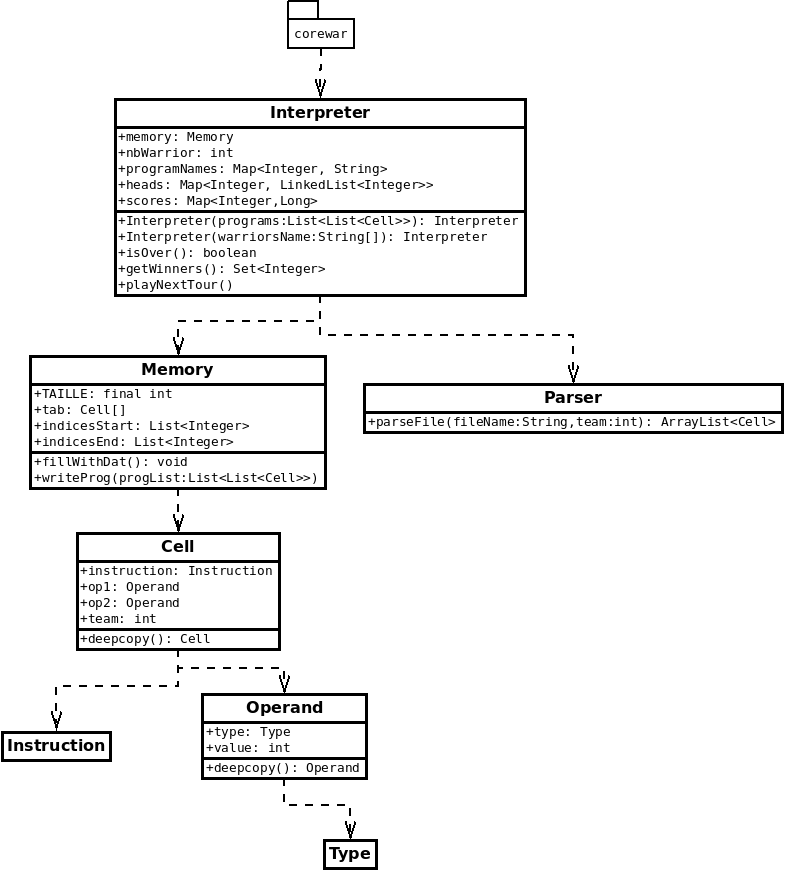
\includegraphics[width=0.9\textwidth]{images/diagram-corewar}
	\caption{Diagramme de classe du package du corewar}
\end{figure}

Le code du CoreWar se situe dans le package Java "corewar". La classe \code{Cell} représente une case de la mémoire virtuelle. Elle est composée d'une \code{Instruction}, de 2 \code{Operand} et d'un entier indiquant l'identifiant du programme à laquelle la cellule appartient. La classe \code{Operand} est en charge de stocker le mode d'adressage (\code{Type}) et l'adresse sur laquelle l'instruction opère. Le code permettant de transformer un fichier RedCode en une suite de cellules correspondant au code des programme se situe dans la classe \code{Parser}. La mémoire virtuelle est représentée par la classe \code{Memory}. Une fois transformé en une liste de cellules, le code d'un programme RedCode est exécuté par la classe \code{Interpreter}.

\subsection{Répartition des tâches}
Pour la première partie du projet, chaque personne s'est vue attribuée une tache spécifique pour être en mesure de faire jouer des programmes RedCode. Abdoulaye s'est occupé du programme principal (la classe \code{Main}). Alexander a créé les classes \code{Instruction}, \code{Operand}, \code{Type}, \code{Cell}, et a commencé à écrire la classe \code{Memory}. Matéo a codé le \code{Parser} et Alix l'\code{Interpreter}.
Dans la deuxième partie du projet, Abdoulaye et Alexander travaillaient sur l'interface graphique tandis qu'Alix et Matéo s'occupaient de l'algorithme génétique.

\subsection{Détail du fonctionnement}
Avant de commencer à exécuter les programmes, les fichiers RedCode doivent être transformés en une suite d'instruction interprétable et inscriptible dans la mémoire virtuelle. Cette tâche est effectuée par le \code{Parser}. Dans le standard ICWS-88 du RedCode, le programmeur à la possibilité d'utiliser des labels et des constantes dans son code. Le \code{Parser} fait donc deux passes: une première pour repérer ces labels et une deuxième qui charge réellement le code, en remplaçant les labels. La norme autorise aussi des opérations arithmétiques sur les adresses mémoires. Le \code{Parser} évalue ces opérations à l'aide d'un interpréteur Java Script. Certaines combinaisons d'instructions et de modes d'adressage sont illégales, par exemple \code{mov 0, #1}. Le \code{Parser} se charge donc de vérifier que toutes les instructions sont correctes avant de charger un programme. Pour éviter qu'un programme remplisse la mémoire par sa taille, les programmes de plus de 100 lignes seront tronqués.

Une fois chargés, les programmes sont écrits dans la mémoire virtuelle. Elle est d'abord remplie d'instructions \code{DAT}, puis les programmes y sont copiés à des emplacements aléatoires. La classe \code{Memory} stocke les indices des positions de début et de fin des programmes pour éviter qu'un programme soit écrit sur un autre.

Une fois les programmes chargés et écrits en mémoire, l'interpréteur créer une file pour chaque programme correspondant à la liste des processus en cours d'exécution. Au départ, elles ne contiennent qu'un seul élément indiquant la position de la première instruction du programme dans la mémoire. Ensuite, la partie peut commencer. On avance d'un tour en appelant la méthode \code{playNextTour} d'\code{Interpreter}. Pour chaque programme, elle récupère le premier élément de sa file d'exécution et vas chercher la case mémoire correspondante. Ensuite, les adresses sont résolues. Si le mode d'adressage est octothorpe, la valeur n'est pas modifiée. S'il est direct, alors la valeur est ajoutée à la position courante du pointeur d'exécution (il s'agit donc d'une adresse relative). S'il est indirect, le résultat est la valeur de la deuxième opérande de la case mémoire pointée par l'opérande courante. Le mode d'adressage peut aussi être en pré-incrémente ou pré-décremente, au quel cas la valeur de la deuxième opérande de la case mémoire pointée est modifiée avant d'être retournée. La mémoire virtuelle est circulaire, sans discontinuité. La case $n-1$ se situe juste avant la case $0$. Les adresses sont donc modulées par la taille totale de la mémoire avant d'être retournées. Une fois les adresses résolues, l'instruction peut être exécutée. Par défaut, la position de l'instruction suivante est ajouté à la fin de la file d'exécution. Cependant, si l'instruction courante est un \code{DAT}, le processus meurt et rien n'est ajouté à la file du programme. Si le programme effectue un saut (via \code{JMP}, \code{CMP}, \code{DJN}, ou autre), la position de l'instruction suivante est modifié avant d'être ajoutée à la file. Si une autre case mémoire est modifiée, elle est marquée comme appartenant au programme courant.

La fonction principale de la classe \code{Main} appelle la méthode \code{playNextTour} tant que que la méthode \code{isOver} de l'interpréteur renvoie faux, c'est à dire tant qu'il reste au moins 2 programmes toujours en vie et que le nombre de tour maximum n'a pas été atteint.
\section{Algorithme Génétique} %% voir si besoin de renommer partie par AG
\subsection{Intoduction}

Une fois un CoreWar fonctionnel, un de nos nouveaux objectifs était de trouver un moyen de générer des programmes automatiquement.
Générer des programmes en RedCode est une chose mais faire que ces programmes soit performant n'est pas si simple. pour se faire, nous avons opté pour une méthode se basant sur un algorithme génétique. Le but étant d'obtenir des programmes s'améliorant après plusieurs générations en se basant sur des mécanismes de modifications, voir de générations, et de sélections avant chaque nouvelle générations.

\begin{figure}[!ht]
	\centering
	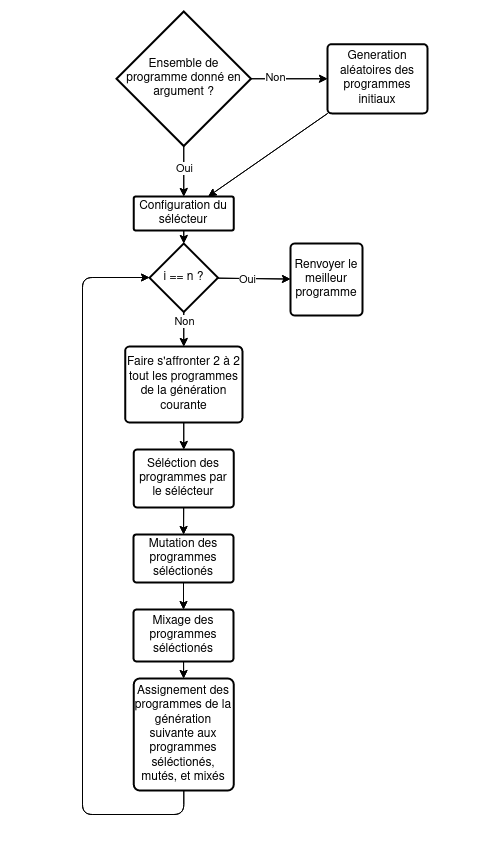
\includegraphics[height=0.5\textheight]{images/schema-algogen}
	\caption{Schema du fonctionnement de l'algorithme génétique}
\end{figure}
\begin{figure}[!ht]
	\centering
	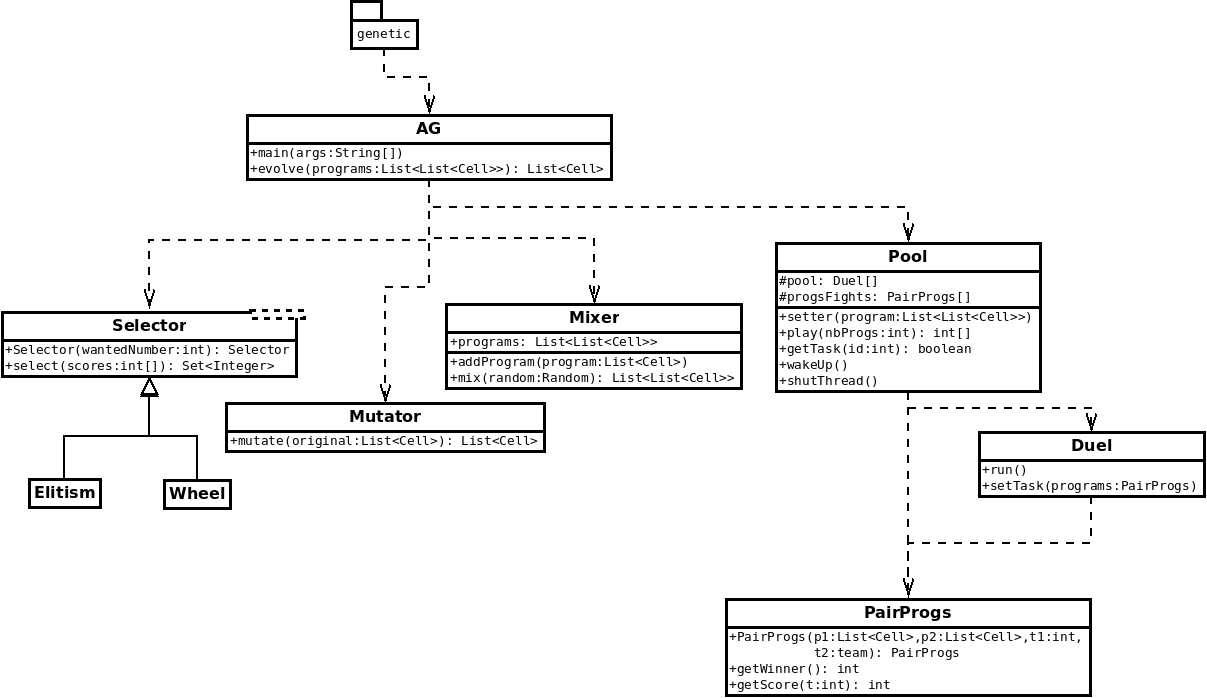
\includegraphics[width=0.9\textwidth]{images/diagram-algogen}
	\caption{Diagramme de classe du package de l'algorithme genetique}
\end{figure}


\subsection{Méthodes de générations}
Afin de générer des nouveaux programmes, nous avons expérimenter 3 méthodes:

\begin{enumerate}
	\item génération aléatoire de séquences d'instructions avec leurs Opérandes.
	\item fusion de deux programmes donnés. (Avec la class \code{Mixer}.)
	\item mutation d'un programme. (Avec la class \code{Mutator}.)
\end{enumerate}

La première s'est montrée inefficace en raison de l'aspect trop aléatoire générant beaucoup d'instructions menant à la mort rapidement du programme. Nous avons donc décidé par la suite de privilégier le chargement de programmes préexistants pour la première population soumise à l'algorithme génétique. Le but étant de passer plus rapidement à l'amélioration de ceux-ci.

La deuxième est l'un des deux processus utilisé pour former une nouvelle population après la sélection réalisée sur la précédentes. Il s'agit de faire muter aléatoirement quelques instructions et opérandes d'un programme.

La troisième est l'autre processus utilisé pour former les nouvelles populations après sélections. Il s'agit de prendre 2 programmes sélectionnées et d'en créer un nouveau en réalisant une fusion en parcourant les cellules de chaque programmes et choisissant de façon stochastique laquelle retenir.


\subsection{Méthodes de sélections}
Au coeur d'une algorithme génétique on retrouve le mécanisme de sélection essentiel pour choisir les individus qui formeront le socle de la génération suivante.
Pour cela on va d'abord évaluer le score de chaque programme de la population : on réalise des duels successif entre tout les programmes 2 à 2 et on leur attribut des points en fonction du résultat du duel et du temps mis pour obtenir cette victoire. Nous évoquerons dans la partie résultats certaines évolutions et leur raison dans ce système d'évalution.

Une fois le score de chaque programmes réalisé, il faut procéder à une sélection de ceux-ci pour former le socle de la population suivante. Pour cela nous avons implémenter 2 mécanisme de sélections:

\begin{enumerate}
	\item Élitisme, réalisée avec la class \code{Elitism}.
	\item Roue, réalisée avec la class \code{Wheel}.
\end{enumerate}

Le premier est le mécanisme le plus simple, il s'agit simplement de prendre les programmes ayant les meilleurs scores de la population.
Et le deuxième procède à une sélection stochastique des programmes en favorisant la sélections des programmes à plus haut scores mais laissant une chance aux autre programmes. L'idée étant que peut-être que ces programmes se trouvait proche d'une solution meilleure mais nécessitant une mutation ou une fusion pour s'en rapprocher.
note : ces 2 classes hérite de la class abstraite \code{Selector} afin de rendre plus générique leur utilisation.

\subsection{Parallélisme}
Une fois notre algorithme génétique implémenté avec nos différents mécanismes, nous avons souhaité réduire le temps de calcul des scores à chaque générations car il s'agit de l'opération la plus coûteuse du processus. Pour celà, on a donc voulu réaliser du parallélisme en implémentant une thread pool.

Le principe fonctionne de la façon suivante : Notre classe \code{Pool} va initialiser et gérer la répartition des tâches des instances de la classe \code{Duel} (qui sont nos Thread). Une fois initialisé, les Threads sont lancé avec la méthode \code{run()} avant de directement se mettre en attente avec \code{wait} avant de recevoir leur tâches.
Pour la lancer ensuite rien de plus simple : tout d'abord on lui fourni la liste des programmes à évaluer (notre population) via sa méthode \code{setter}, avant de la lancer pour en récupérer les scores une fois que celle-ci à fini avec sa méthode \code{play}.
Une fois lancée, cette méthode va réveiller chacun des threads avant de s'endormir (là aussi avec \code{wait()} et un petit mécanisme pour s'assurer de se rendormir si jamais un ou plusieurs autre thread n'a pas fini son travail).
Les Threads étant réveillé vont faire appelle à la méthode \code{getTask} de la pool qui va leur indiquer si oui ou non il leur reste du travail à réaliser dans la pile de travail de la pool, et si c'est le cas va leur fournir directement ce travail.
Quand ils n'ont plus de tâche à réaliser, ils envoient leur signal de réveil à la pool et retourne se mettre en attente avant la prochaine population à évaluer.
Une fois tous les threads terminé, la pool sort de son attente pour calculer et retourner les scores de la population actuelle à l'algorithme génétique.
Une fois l'algorithme génétique terminé, il appelle la méthode \code{shutThread} de la pool, qui la envoyé un signal à ses threads pour leur dire de se terminer, afin d'éviter d'avoir des processus perdus malgré la fin du programme principal.

La difficulté fût ici est d'obtenir une synchronisation entre les threads et la pool lors de l'arrivé de nouvelles tâches et quand les threads avaient fini des les traiter. C'est ce qui nous a mener à l'utilisation des méthodes \code{wait} et \code{notify}.

\subsection{Résultats}
Au cours de notre implémentation nous avons pu observer différents premiers résultats lié à l'ajout ou le retrait des mécanisme évoqué précédement. Avant de pouvoir expérimenter avec notre dernière version de l'algorithme génétique.

Notre premier algorithme génétique fonctionnel consistait à l'implémentation de 3 mécanismes de base: 1 de sélection et 2 de génération. Il s'agissait de la sélection par élitisme, de la génération complétement aléatoire des programmes constituant la population initiale et de la
Au début, nous avions implémenté seulement quelques mécanismes: tout d'abord la génération complétement aléatoire de programmes pour générer la population initiale et pour terminer le mécanisme de mixage pour former les populations suivantes à partir de celles sélectionnées. 
Dès lors, nous avons pu observer un phénomène de consanguinité. En effet, après une centaine de générations, nous commencions à obtenir des programmes de plus en plus similaire avant de finir par l'obtention d'un seul programme, qui plus est dégénéré, comme constituant de chaque individu de chaque population suivante. Cela s'explique par le nom renouvellement aléatoire des programmes ou au moins d'une partie des programmes, couplé avec le mode de génération par fusion utilisé seul pour générer de nouvelle population, on fini donc par tendre inéxorablement vers un programme unique comme résultat, par particulièrement bon non plus en raison de la génération trop aléatoire de la population initiale. 
La première chose que nous avons décider de faire pour pallier à ce phénomène a été d'introduire une nouvelle génération de quelques programmes aléatoires à chaque génération de population afin de régénérer le potentiel d'évolution à chaque nouvelle génération. De plus, nous avons en même temps mis au point le mécanisme de mutation et décider de l'introduire là encore dans la génération de population.
Cela à en partie fonctionné, mais là encore, en raison du caractère trop aléatoire de la génération de la population de départ, nous n'obtenions pas de résultat très intéressant: les programmes avaient tendance à devenir les plus long possible et ne survivaient que ce qui arrivaient de s'éliminer eux même en plus de temps de les autres. Cela aurait peut-être pu donner des résultat, mais pas avant de très très nombreuses générations et là encore sous-réserve d'avoir de la chance.

Nous avons donc décidé de faire 2 choses: supprimmer la composante de génération de nouveau programmes totalement aléatoire dans la formation de chaque nouvelle population, et de charger des programmes préexistant comme population initiale. L'objectif étant de donner un rôle d'optimisation de programmes à l'algorithme génétique, évitant par conséquent la partie recherche de stratégie ou de programme un minimum fonctionnel qui aurait été beaucoup trop chronophage.
En plus de cela, nous avons implémenté la sélection stochastique avec la roue.
\\ \\
Récapitulons, nous avons donc maintenant un algorithme génétique qui : 
\begin{itemize}
	\item Charge des programmes préexistant comme population initiale.
	\item Bénéficie d'une méthode de sélection par élitisme ou par roue, au choix.
	\item Possède un mécanisme de mutation et de fusion pour la génération des populations suivantes.
\end{itemize}

En parallèle de l'algorithme, nous avons permis à celui-ci de pouvoir écrire directement dans un fichier ses résultats avec la création de la class \code{CellToFile}.

Une fois cet partie implémenté, nous l'avons donc testé avec des programmes que nous avions réalisé et nous avons pu constat le résultat suivant: les programmes obtenus étaient plus performant après un dizaine de génération qu'après une centaine, un millier, ou plus, de générations. Nous avions un peu anticipé une partie de ce phénomène lors de la réalisation de la partie évalution des programmes qui consister à un simple tableau des scores auquel on ajouter un point au score de chaque programme lorsqu'il l'emporter contre un autre. Et ce malgré le fait que le programme ait pu bénéficier un coup de chance en raison de sa position relative à son adversaire. Nous avons donc décider d'augmenter le nombre de duel entre 2 programmes afin d'obtenir une moyenne du résultat de ces affrontements. 

Cela permis d'améliorer un peu les résultats obtenus au delà de la centaine de génération mais pas énormément. Notre conclusion est que en effet, ce calcul ne prend pas en compte la valeur d'un score en fonction de l'adversaire. En effet, il est simple d'obtenir de multiple victoire consécutive contre des programmes dégénérés mais une victoire contre un autre programme fort est plus difficile à obtenir. Pour résoudre cela, plusieurs options s'ouvre à nous, mais nous n'avons pu en implémenter qu'une faute de temps: nous pourrions ajouter un poids relatif au nombre de cycle menant à l'obtention d'une victoire lors des affrontements (ce que nous avions commencé à faire).

Cet fois, on a pu observer une net amélioration car cette fois nous obtenions des programmes fonctionnel et capable de rivaliser un peu contre les programmes initiaux et à gagner contre au moins la moitié d'entre eux de façon constante. On observe aussi chez eux des stratégies qui peuvent totalement différer des programmes initiaux.

Afin d'évaluer plus proprement ces résultats, nous avons décider d'implémenter un évaluateur de programmes, avec la class \code{Benchmark}, sur différentes métriques simples:
\begin{enumerate}
	\item Le nombre de cycle de survie d'une programme par lui-même. (Pour évaluer si le programme ne va pas se tuer lui-même dès le début ou savoir si à terme il finit par s'attaquer lui-même.)
	\item Sa fréquence d'écriture d'autre case qui ne lui appartiennent pas. (Pour évaluer sa vitesse d'attaque.)
	\item Le pourcentage final d'occupation de la mémoire. (Pour évaluer sa force d'occupation.)
	\item Son nombre de split (exécution de l'instruction SPL pour créer de nouveaux processus) et combien reste en vie au cours du temps. (Pour évaluer sa vulnérabilité aux attaques adverses.)
	\item Le nombre de case total qu'il va écrire sur un nombre donné de cycle.
	\item Le nombre de bloque de 5 Cellules qu'il aura exploré lors de ces écritures. (Car écrire rapidement en ligne droite et parfois moins intéressant que d'écrire en ligne droite avec un pas plus élevé.)
\end{enumerate}

Nous sommes conscients qu'il existe d'autres métriques intéressantes, voir une infinité, et que baser notre vision sur celle-ci va forcément créer un biais dans les statégies que l'on va favoriser. Et finalement, nous l'avons assez bien observé avec les résultats récolté par notre benchmark:

\newpage

\begin{figure}[!ht]
\centering
\begin{minipage}{.5\textwidth}
  \centering
  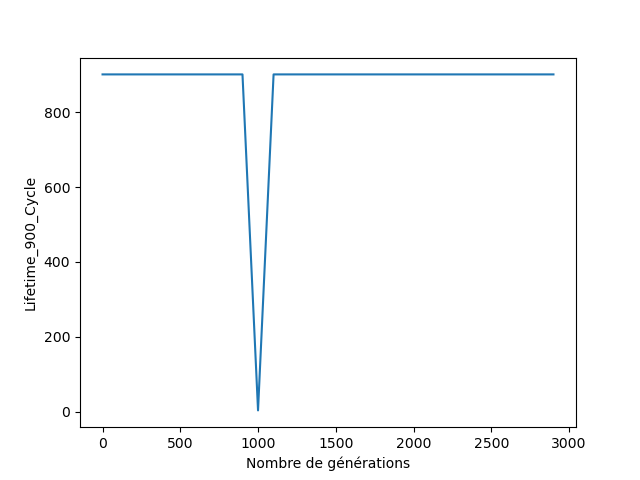
\includegraphics[width=.5\linewidth]{images/Lifetime_900_Cycle.png}
%  \captionof{figure}{Nombre de cycle de survie d'un programme sur 900 cycle.}
  \label{fig:test1}
\end{minipage}
\begin{minipage}{.5\textwidth}
  \centering
  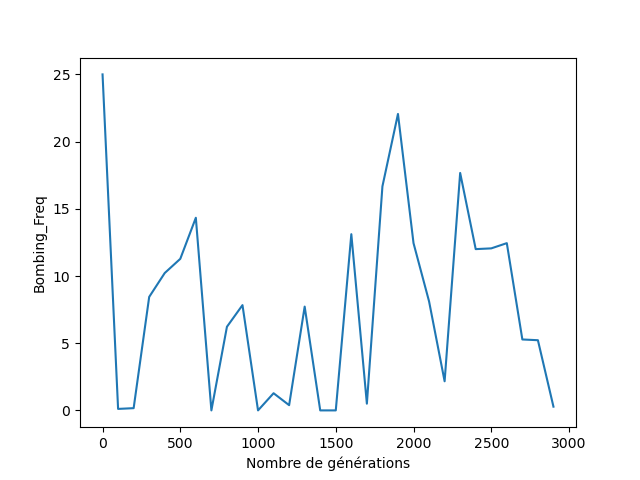
\includegraphics[width=.5\linewidth]{images/Bombing_Freq.png}
%  \captionof{figure}{Moyenne du nombre de cases écrites tout les 50 cycles.}
  \label{fig:test2}
\end{minipage}
\begin{minipage}{.5\textwidth}
  \centering
  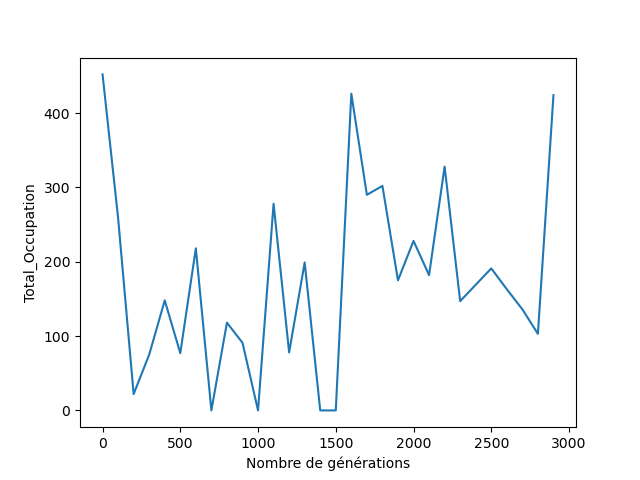
\includegraphics[width=.5\linewidth]{images/Total_Occupation.png}
%  \captionof{figure}{Nombre de cases écrites sur 900 cycles.}
  \label{fig:test3}
\end{minipage}
\begin{minipage}{.5\textwidth}
  \centering
  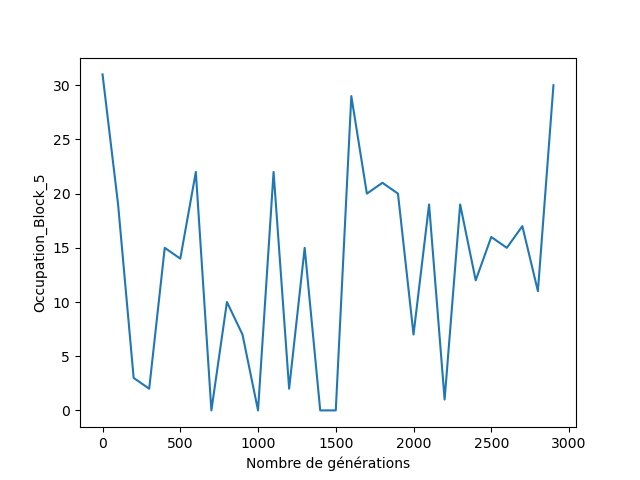
\includegraphics[width=.5\linewidth]{images/Occupation_Block_5.png}
%  \captionof{figure}{Nombre de bloque de 5 cellues exploré sur 900 cycles.}
  \label{fig:test4}
\end{minipage}
\begin{minipage}{.5\textwidth}
  \centering
  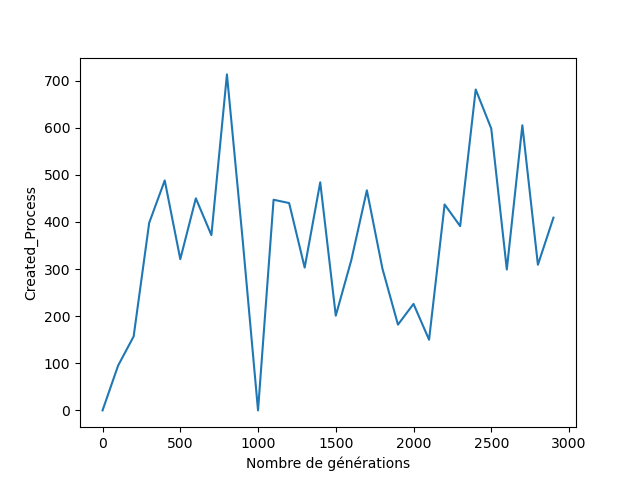
\includegraphics[width=.5\linewidth]{images/Created_Process.png}
%  \captionof{figure}{Nombre de processus crée sur 900 cycles.}
  \label{fig:test5}
\end{minipage}
\begin{minipage}{.5\textwidth}
  \centering
  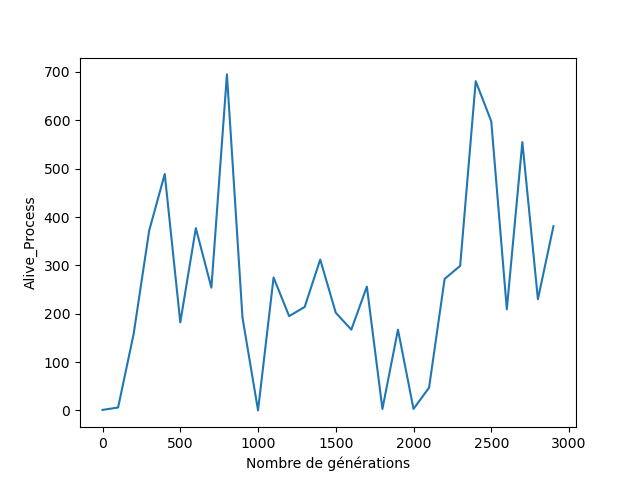
\includegraphics[width=.5\linewidth]{images/Alive_Process.png}
%  \captionof{figure}{Nombre de processus en vie après 900 cycles.}
  \label{fig:test6}
\end{minipage}

\end{figure}

On remarque une évolution ératique des différetentes métriques hormis celle du temps de survit seul (à l'exception des valeurs abérentes).
Ce qui nous fait dire que le Benchmark n'est a utilisé en priorité que pour essayer d'améliorer une stratégie particulière dont on a déterminé les bonnes métriques.

\section{Interface graphique}

\subsection{Objectifs}

L'objectif était de créer une interface graphique simple avec un affichage des cellules de la mémoire, les cellules occupées par les programmes dans différentes couleurs et les têtes de lecture de chaque programme, ainsi que le nom des programmes qui combattent. (\ref{jeu})
Nous voulions aussi créer un menu (\ref{menu}) nous permettant de sélectionner les programmes à faire combattre.\\
Ce menu est composé de 4 boutons qui sont le bouton valider qui valide les programmes saisis, le bouton vider le champs qui efface la zone de saisie des programmes, le bouton jouer pour lancer le jeu et le bouton quitter pour quitter le menu.

\subsection{Difficultés rencontrées}

Nous avions rencontré des difficultés sur la transition entre le menu ou nous sélectionnons les programmes à faire combattre et l'interface graphique où les programmes se combattent car l'interface ne se rafraîchissait pas mais le problème venait du fait qu'il y avait une instruction bloquante en liste d'attente de awt.

\subsection{Ce qu'on a réussi et ce qu'on pourrait ajouter}

Nous avons donc une interface graphique qui affiche les programmes qui combattent à une vitesse normale. Nous avons également un menu ou nous pouvons sélectionner les programmes à faire combattre qui nous ramène vers le jeu où nous faisons combattre ces programmes. 

Nous pourrions rajouter le nom des programmes qui combattent, des boutons nous permettant de modifier la vitesse des combats ou pauser le combat ainsi que les statistiques de chaque programme.

Nous aurions également pu afficher les cellules sous forme circulaire pour avoir une meilleure représentation de l'occupation de la mémoire par les programmes.

\newpage
\subsection{Résultat final}
\begin{figure}[hb]
\centering
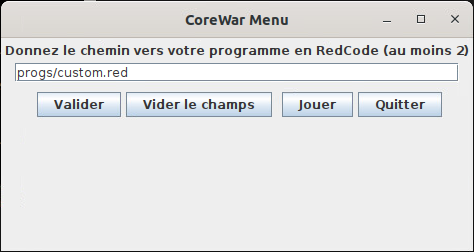
\includegraphics[scale=0.6]{images/mainMenu.png}
\captionof{figure}{Menu principal}
\label{menu}

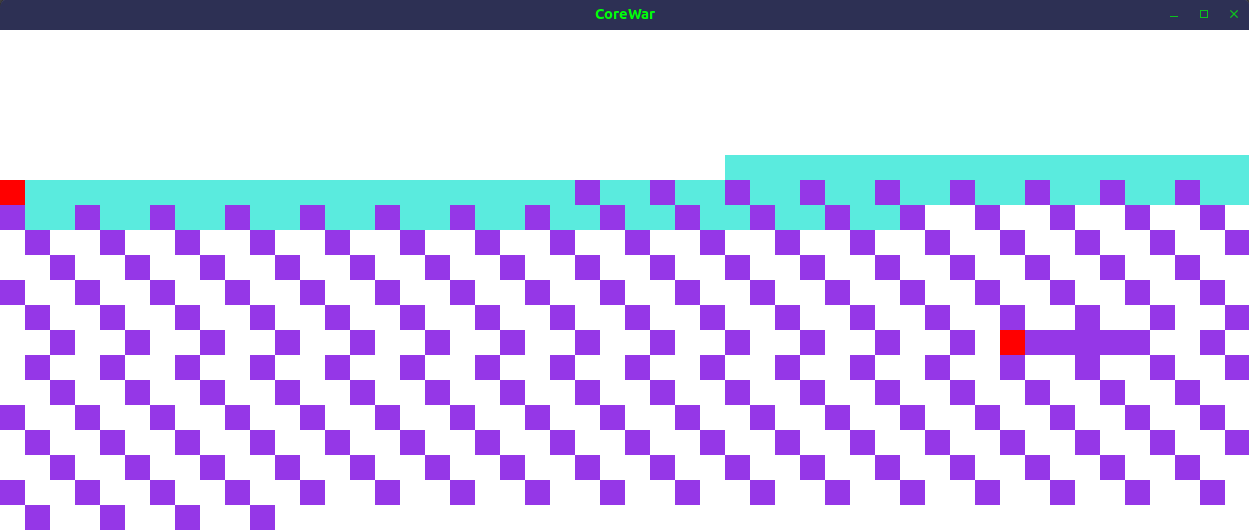
\includegraphics[scale=0.3]{images/jeu.png}
\captionof{figure}{Jeu}
\label{jeu}

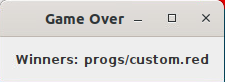
\includegraphics[scale=0.7]{images/gameOver.png}
\captionof{figure}{Fin de jeu avec affichage du gagnant}
\label{over}
\end{figure}

\newpage
\section{Conclusion}

La partie CoreWar est fonctionnelle. L'interface graphique est très simple mais également fonctionnelle. L'algorithme génétique permet de générer des programmes qui gagnent face à nos programmes écrits manuellement.

\subsection{Pistes d'évolution du CoreWar}
Notre implémentation actuelle du CoreWar suit la norme ICWS-88. Il pourrait être possible d'étendre le support à des normes plus récentes, tel que l'ICWS-94. On pourrait aussi envisager une communication par socket entre l'interpreteur et l'interface graphique. Cela permetterait de visualiser des parties distantes et d'avoir plusieurs interfaces graphiques pour un seul interpreteur.

\subsection{Pistes d'amélioration de l'algorithme genetique}
Afin d'optimiser les performances des programmes générés avec l'algorithme génétique, on pourrait essayer d'assigner une valeur à chaque programme d'une génération en fonction de diverses critères, tel que le nombre de case mémoire écrites, le nombre de processus créés, de processus morts... Cette valeur viendra pondérer les scores des programmes lors de leurs affrontements: un programme qui bat un programme de valeur 10 aura un meilleur score que s'il bat un programme de valeur 1. Cette méthode pourrait peut être affiner la séléction des programmes afin de les améliorer plus rapidement.

Une autre piste serait de faire varier les addresses des instructions des programmes d'une génération, comme le fait actuellement le \code{Mutator} mais uniquement sur les addresses. Cela permetterait peut-être d'augmenter les chances de créer des programmmes cohérents qui intéragissent avec eux même au lieu de faire des \code{SPL} et des \code{CMP} à des endroits aléatoire de la mémoire.

La méthode de fusion des programmes pourrait également être revue. Actuellement, chaque cellule du programme final est choisit aléatoirement parmis l'une des cellules des deux autres programmes à la même position. On pourrait aussi imaginer une fusion bout-à-bout, où des blocs entier de programme serait mis à la suite.


\end{document}
